\documentclass[preprint,12pt,authoryear]{elsarticle}
% Target: Applied Soft Computing (Elsevier).  Compile with pdflatex + bibtex (e.g. Overleaf).
% Tables and in-text numbers are generated: run experiments/make_tables.py and experiments/make_figures.py.

\usepackage{amsmath,amssymb}
\usepackage{booktabs}
\usepackage{graphicx}
\usepackage{xcolor}
\usepackage[hidelinks]{hyperref}
\usepackage{xspace}
\graphicspath{{figures/}}
% generated by experiments/make_tables.py -- do not edit
\newcommand{\EEightCD}{4.00}
\newcommand{\EEightRank}{4.22}
\newcommand{\EEightRulesMax}{15}
\newcommand{\EEightRulesMin}{3}
\newcommand{\EOneCD}{2.89}
\newcommand{\EOneCov}{0.960}
\newcommand{\EOneMAE}{52.4}
\newcommand{\EOneRank}{5.09}
\newcommand{\EOneSA}{0.368}
\newcommand{\ETwoCov}{0.945}
\newcommand{\ETwoMAE}{36.6}
\newcommand{\ETwoWidth}{29}
\newcommand{\MonoMax}{100}
\newcommand{\MonoMin}{92}
\newcommand{\ProxyIssues}{9,054}
\newcommand{\ProxyPositive}{15}
\newcommand{\ProxyProjects}{15}
\newcommand{\ProxyRho}{0.35}
\newcommand{\ProxyRhoHi}{0.44}
\newcommand{\ProxyRhoLo}{0.14}
\newcommand{\RulesMax}{36}
\newcommand{\RulesMin}{27}
\newcommand{\SBGain}{0.46}
\newcommand{\SBp}{8e-09}
\newcommand{\StableSame}{74}
\newcommand{\StableWithinOne}{100}


\newcommand{\dynest}{DynEst-R\xspace}
\newcommand{\todo}[1]{\textcolor{red}{[TODO: #1]}}

\journal{Applied Soft Computing}

\begin{document}

\begin{frontmatter}

\title{What does transparency cost? A fully data-trained neuro-fuzzy effort estimator\\
evaluated on agile issue histories and classic benchmarks}

\author{\todo{author names and affiliations}}

\begin{abstract}
Neuro-fuzzy effort estimators promise accuracy with explanations, but their rule bases are usually written by hand,
their evaluations use small datasets and random splits, and their interpretability is asserted rather than measured.
We present \dynest, a pipeline in which every component is learnt from real data: a self-organising map (SOM) supplies
an empirical-Bayes prior from similar past work, an ANFIS model learns a complexity score, and a Mamdani system whose
rules are generated by Wang--Mendel learning and whose partitions are tuned by a genetic algorithm maps its inputs to
effort; split-conformal prediction adds 95\% intervals.  A transparent variant, \dynest-T, feeds the rules only
named, measured inputs.  We evaluate on 21,928 requirements from 22 open-source agile projects whose features are
reconstructed \emph{as of the moment work started} from the Jira change log, with effort measured from status
histories and validated against logged work time (median Spearman $\rho=\ProxyRho$, positive in
\ProxyPositive/\ProxyProjects{} projects), on the same projects held out one at a time, and on nine classic Function
Point and COCOMO datasets.  Every model receives the same tuning budget and the same interval method.  \dynest-T
explains each estimate with a rule base of \TRulesMin--\TRulesMax{} rules over three named inputs, and
\TMonoMean\% of neighbouring rules move in directions declared before the experiment.  This transparency costs about
one per cent of accuracy: \dynest-T reaches \ElevenMAEt{} hours mean absolute error against \ElevenMAEGBM{} for tuned
gradient boosting, the same as an Explainable Boosting Machine (\ElevenMAEEBM), better than a depth-limited tree, and
no worse than fine-tuned GPT-2 and DeBERTa-v3 text regressors.  It is more accurate than CAEA and story-point
velocity on agile data and than COCOMO-81 on independent data.  Every model's intervals reach nominal coverage under
the shared recipe, so calibration is a property of the method, not of the model.  We release code, protocol and the
pre-registration with its amendment.
\end{abstract}

\begin{keyword}
software effort estimation \sep neuro-fuzzy systems \sep ANFIS \sep self-organising map \sep Mamdani fuzzy inference
\sep interpretability \sep conformal prediction \sep agile development
\end{keyword}

\end{frontmatter}

%==================================================================================================
\section{Introduction}
\label{sec:intro}

Software effort estimates drive staffing, commitments and scope decisions, yet the models used to produce them are
either opaque (tree ensembles, neural networks, fine-tuned language models) or rest on constants and rules fixed by
experts decades ago (COCOMO, Function Point productivity tables, hand-written fuzzy rule bases).  Soft computing has
long promised a middle ground: neuro-fuzzy models that learn from data yet explain their output in linguistic
rules~\citep{huang2007neurofuzzy}.  In practice four gaps keep that promise from being tested.

\emph{First, the rule bases are rarely learnt}, so the readable part of the model encodes the designers' beliefs
rather than evidence.  \emph{Second, readability is assumed, not measured}: rules often read a latent score
produced by another network, and few studies check whether the rules make sense.  \emph{Third, the evaluation rarely
matches use}: small datasets, random cross-validation, unequal tuning budgets, and, in agile studies, the issue's
\emph{final} text, which can be edited after the estimate was made~\citep{tawosi2023deepse}.  \emph{Fourth,
uncertainty is missing}, although a single number is of limited use for commitment decisions.

We address all four and ask a direct question: \emph{how much accuracy does a fully readable, fully learnt fuzzy
rule base cost, compared with the best black-box, glass-box and fine-tuned text estimators, when they are compared
fairly?}  Our contributions are:
\begin{enumerate}
  \item \textbf{A fully data-trained SOM$\rightarrow$ANFIS$\rightarrow$Mamdani pipeline} (\dynest) and a transparent
  variant (\dynest-T) whose rules read only named, measured inputs.  No rule, membership function or effort
  multiplier is written by hand.
  \item \textbf{A decision-time evaluation on real agile histories}: features rebuilt from the Jira change log as of
  the moment work started; effort measured from status intervals with work-in-progress sharing and validated against
  logged time.
  \item \textbf{A fair comparison} against black-box (ridge, random forest, gradient boosting, MLP), glass-box (EBM,
  shallow tree), text (fine-tuned GPT-2 and DeBERTa-v3) and traditional (story-point velocity, COCOMO, CAEA,
  Function Point regression, analogy) estimators, with equal tuning budgets and one interval
  method for all, on agile data and on nine classic datasets.
  \item \textbf{Measured interpretability}: rule-base size and coverage, stability over time, and agreement with
  expected directions declared before the experiment.
\end{enumerate}
The answer is about one per cent of mean absolute error against the best black box, the same price as the leading
glass-box alternative.

%==================================================================================================
\section{Related work}
\label{sec:related}

Machine learning for effort estimation has been surveyed extensively~\citep{wen2012slr}; ensembles and locality
\citep{minku2013ensembles} and multi-objective search~\citep{sarro2016coGEE} are among the strongest learned
approaches on project-level data.  We focus on the four threads closest to our contribution; Table~\ref{tab:related}
positions the most similar studies.

\paragraph{Neuro-fuzzy and fuzzy-rule estimators}
ANFIS~\citep{jang1993anfis} and Mamdani inference~\citep{mamdani1975} have been used for effort estimation for over
two decades.  A common design keeps a parametric model's structure and lets a neuro-fuzzy layer adjust it:
\citet{huang2007neurofuzzy} embed COCOMO's effort multipliers in a neuro-fuzzy network, and \citet{du2015seersem}
do the same for SEER-SEM.  These models gain accuracy over the parametric model while keeping its interpretable
structure, but that structure, and often the rule base, is fixed by the designers rather than learnt.  Fuzzy
analogy~\citep{idri2002fuzzyanalogy} represents project attributes as linguistic values and retrieves similar
projects.  Recent work tunes ANFIS with metaheuristics: \citet{arora2022anfis} optimise ANFIS parameters with an
energy-efficient bat algorithm for Scrum projects, using 21 projects expanded with k-means SMOTE to 162 records.
Such studies typically evaluate on small datasets, sometimes enlarged with synthetic records, against other
metaheuristics rather than against strong tuned regressors under equal budgets.  Genetic fuzzy
systems~\citep{herrera2008ga_fuzzy} learn partitions and rules by evolutionary search, and Wang--Mendel
learning~\citep{wang1992mendel} generates rules directly from data; we combine both so that no rule is
hand-written, and we measure interpretability (size, coverage, stability, domain consistency) rather than assume it.

\paragraph{Clustering before estimation}
Self-organising maps~\citep{kohonen1990som} have been used to group projects before building estimation models,
with SOM-based models outperforming linear regression in case studies~\citep{dai2011som}; locality-based ensembles
pursue the same idea with other clusterers~\citep{minku2013ensembles}.  We use the SOM differently: as an
unsupervised map whose neurons carry an empirical-Bayes prior, computed out-of-fold and passed to ANFIS as a feature,
so the cluster informs the estimate without partitioning scarce data.

\paragraph{Agile and text-based estimation}
Deep-SE~\citep{choetkiertikul2019deepse} and GPT2SP~\citep{fu2022gpt2sp} estimate story points from issue text.
Replications on the TAWOS dataset~\citep{tawosi2022tawos} found that neither is reliably better than simple mean or
median baselines~\citep{tawosi2023deepse,tawosi2022gpt2sprep}.  Large language models are now being tried, through
optimised few-shot examples~\citep{tawosi2023llmshots} and multi-agent Planning-Poker
simulations~\citep{bui2025seeagent}.  These studies predict story points from the issue's final text.  We instead
estimate \emph{effort in hours}, treat the team's story points as an input known at decision time, and rebuild every
feature from the change log as of the moment work started; we include fine-tuned GPT-2 and DeBERTa-v3 regressors
as text-based baselines.  LLM-based estimation is promising but its evaluation under decision-time features is
left to future work (Section~\ref{sec:conclusion}).

\paragraph{Glass-box models}
Interpretable machine learning offers alternatives to fuzzy rules.  Generalised additive models with pairwise
interactions, implemented as Explainable Boosting Machines~\citep{lou2013ga2m,nori2019interpretml}, are often as
accurate as tree ensembles while exposing one shape function per feature.  An interpretability claim for a fuzzy
estimator should be tested against such models, not only against black boxes; we include EBM and a depth-limited
regression tree.

\paragraph{Uncertainty}
Split-conformal prediction~\citep{vovk2005,lei2018conformal,angelopoulos2023gentle} gives finite-sample coverage under
exchangeability.  \citet{andreou2009conformal} applied conformal predictors built on ridge regression to COCOMO,
Desharnais and ISBSG data, and \citet{song2019interval} predicted effort intervals with Bayesian inference and
synthetic bootstrap resampling.  Neither compares interval quality across competing estimators under one recipe; we
give every model the same normalised, cluster-wise conformal interval, which separates the effect of the model from
the effect of the interval method.

\begin{table*}[t]
\centering
\scriptsize
\caption{Positioning against the closest prior work.  \checkmark{} = present; -- = absent or not reported.}
\label{tab:related}
\begin{tabular}{lcccccc}
\toprule
Study & Rules learnt & Real data only & Agile issue data & Decision-time features & Intervals & Strong tuned baselines \\
\midrule
\citet{huang2007neurofuzzy} & partly & \checkmark & -- & -- & -- & -- \\
\citet{du2015seersem} & partly & \checkmark & -- & -- & -- & -- \\
\citet{arora2022anfis} & -- & -- (SMOTE) & \checkmark{} (21 projects) & -- & -- & -- \\
\citet{andreou2009conformal} & -- & \checkmark & -- & -- & \checkmark & -- \\
\citet{song2019interval} & -- & \checkmark & -- & -- & \checkmark & \checkmark \\
\citet{fu2022gpt2sp} & -- & \checkmark & \checkmark & -- & -- & -- \\
\citet{tawosi2023deepse} & -- & \checkmark & \checkmark & -- & -- & \checkmark \\
This work & \checkmark & \checkmark & \checkmark & \checkmark & \checkmark{} (all models) & \checkmark \\
\bottomrule
\end{tabular}
\end{table*}

\paragraph{Evaluation practice}
We follow \citet{shepperd2012sa} in reporting standardised accuracy against random guessing, \citet{demsar2006} for
multi-dataset comparison, and Holm's correction~\citep{holm1979} with paired effect sizes.

%==================================================================================================
\section{Method}
\label{sec:method}

\subsection{Overview}
\dynest predicts the logarithm of effort per unit of size (hours per story point on agile data, effort per FP or
KLOC on classic data); size enters as a known offset, so the fuzzy stages model productivity rather than scale.
The pipeline has six stages, all fitted on the training window only.

\paragraph{S1 Measured features.}  On agile data: story points, issue type and priority, number of components and
links, description length and acceptance-criteria presence, assignee familiarity with the components, and a 16-d PCA
projection of a frozen MiniLM sentence embedding~\citep{reimers2019sbert} of the as-of title and description.  On
classic data: the dataset's own predictors, with skewed predictors log-transformed and categorical predictors
one-hot encoded inside each training fold.

\paragraph{S2 Learnt attributes (agile data).}  Gradient-boosting models trained on training-window labels estimate
requirement clarity and integration load; non-negative matrix factorisation of component usage yields topic profiles.

\paragraph{S3 SOM cluster prior.}  A SOM is trained on the text, profile and integration features.  Each neuron $j$
stores a shrunk prior of the target, $\pi_j = (n_j\bar{y}_j + m\,\bar{y})/(n_j+m)$, with $m$ tuned on validation.  The
prior fed to the next stage is computed out-of-fold so that ANFIS never sees a row's own target through its cluster.

\paragraph{S4 ANFIS complexity score.}  A first-order Sugeno ANFIS~\citep{jang1993anfis} with Gaussian memberships
maps the prior and the top-ranked predictors to a score $\hat c$ (hybrid learning: ridge least squares for the
consequents, gradient descent for the premises, early stopping on validation).  $\hat c$ for the next stage is again
out-of-fold.  Consequents support recursive least-squares updates for online use.

\paragraph{S5 Learnt Mamdani system.}  Inputs $\hat c$, clarity and familiarity (agile) or $\hat c$ and the
next-ranked predictors (classic) are covered by strong triangular partitions, so memberships of adjacent terms sum to
one and every input is covered.  Rules are generated by Wang--Mendel learning~\citep{wang1992mendel} with a
membership-weighted mean consequent (a majority vote over output terms collapses noisy data onto the middle term) and
a minimum-support threshold.  A real-coded genetic algorithm (BLX-$\alpha$ crossover, tournament selection, elitism)
moves the partition centres; rules are regenerated for each candidate and fitness is MAE on an internal hold-out.
Inference uses min-AND, min-implication, max-aggregation and centroid defuzzification.

\paragraph{Transparent variant (\dynest-T).}  In the full pipeline the Mamdani system's first input is the latent
score $\hat c$, so a rule such as ``IF $\hat c$ IS low \dots'' is only as readable as ANFIS.  \dynest-T instead feeds
the Mamdani system the SOM prior, which reads as ``hours per story point of similar past work in this project'', and
the two measured, non-binary features most related to the target on the training window (absolute Spearman
correlation); ANFIS is not used.  On TAWOS this selection chose familiarity of the assignee with the components and
the story-point count in every origin, so every rule reads in domain terms, for example ``IF similar work was slow AND
the assignee is unfamiliar AND story points are low THEN hours per point are high''.

\paragraph{S6 Back-transform and intervals.}  Predictions are mapped back to effort with a shift $s$ learnt on
validation: the weighted median of $\log(y/\hat y)$ with weights $\hat y$, which minimises validation MAE (a
mean-unbiased smearing correction inflates estimates under heavy tails).  Intervals are normalised split-conformal:
a gradient-boosting model of $|\text{residual}|$ is trained on the first half of the validation window, score quantiles
are taken on the second half, per SOM cluster when it has $\ge$30 points.

Hyper-parameters (SOM grid and shrinkage, ANFIS inputs and memberships, Mamdani terms, output terms and support) are
chosen by random search on validation MAE.  Ablation switches remove each stage (Section~\ref{sec:design}).

%==================================================================================================
\section{Data and measurement}
\label{sec:data}

\subsection{Agile issue histories (TAWOS)}
TAWOS~\citep{tawosi2022tawos} contains 458k issues and 9.25M change-log rows from 39 Jira projects.  We parse the
public SQL dump directly.  A project enters the study if it has at least 150 modelling rows and 10 sprints, giving 22
projects and 21,928 resolved requirements.

\paragraph{Decision time.}  TAWOS' estimation timestamp is an artefact (one hour before creation), so we set the
decision time to one second before work first started (first transition into an active status).  Every feature is
reconstructed from the change log as of that instant; labels used to train S2 are computed as of resolution.

\paragraph{Effort proxy and its validity.}  Few issues carry logged time, so effort is measured: business hours spent
in active statuses, with each assignee's time shared equally across their concurrently active issues.  To test
construct validity we recomputed the proxy for the \ProxyProjects{} TAWOS projects with at least 50 resolved issues
carrying logged work time (\ProxyIssues{} issues) and correlated it with that logged time
(Figure~\ref{fig:proxy}).  The median Spearman correlation is \ProxyRho{} (BCa 95\% CI \ProxyRhoLo--\ProxyRhoHi),
positive in \ProxyPositive{} of \ProxyProjects{} projects, at least as high as TAWOS' own in-progress and total-effort
minutes and well above cycle time.  The proxy is therefore a noisy but valid measure of work, and part of the
irreducible error reported below is measurement noise.

\begin{figure}[t]
\centering
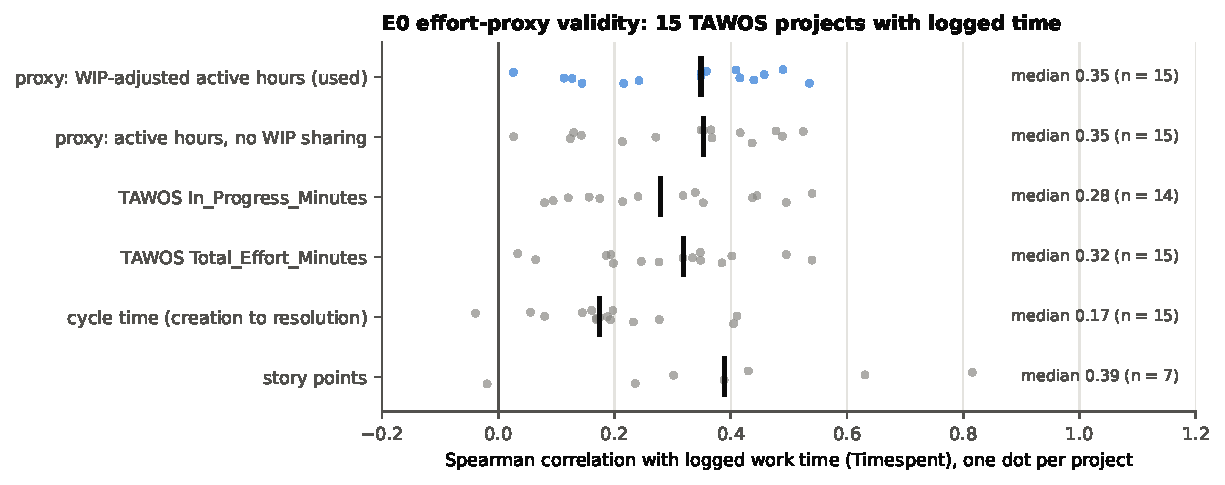
\includegraphics[width=\linewidth]{fig_proxy}
\caption{Construct validity of the effort proxy: per-project Spearman correlation with logged work time.}
\label{fig:proxy}
\end{figure}

\subsection{Classic project-level datasets}
We use the public PROMISE copies of Albrecht~\citep{albrecht1983} (24 projects), Kemerer~\citep{kemerer1987} (15), Desharnais (77 complete), China (499),
Maxwell (63), Kitchenham (145), Miyazaki94 (48), COCOMO81 (63) and NASA93 (93).  Columns known only after a project
ends (actual duration) are removed.  NASA93's ordinal COCOMO ratings are converted with the multiplier table
recovered from COCOMO81, which ships both encodings of the same projects; the recovered table equals Boehm's
published values~\citep{boehm1981}.  Kitchenham's recorded first human estimate is kept as a reference, not a
predictor.

%==================================================================================================
\section{Experimental design}
\label{sec:design}

\paragraph{Research questions.}
\textbf{RQ1} What accuracy do fully readable learnt fuzzy rules cost, relative to strong black-box, glass-box and
fine-tuned text estimators, on later requirements of the same agile projects?
\textbf{RQ2} Does the pipeline generalise to projects it has never seen?
\textbf{RQ3} How does it compare with Function Point and COCOMO models on classic project-level datasets?
\textbf{RQ4} What does each stage contribute?
\textbf{RQ5} Are its intervals calibrated, relative to baselines given the same interval recipe?
\textbf{RQ6} Are the learnt rules compact, stable and consistent with domain knowledge declared in advance?

\paragraph{Splits.}  TAWOS: per project, three rolling origins at 55/65/75\% of the time-ordered history, followed by
a 10\% validation and a 10\% test window, with a 14-day gap; leave-one-project-out for RQ2.  Classic: 3$\times$10-fold
cross-validation per dataset with the same folds for every model (repeated rather than leave-one-out
validation~\citep{kocaguneli2013loo}, because every model is tuned by an inner cross-validation).

\paragraph{Tuning budget.}  Every tuned model receives the same random-search budget: 40 trials scored on the
validation window on TAWOS (experiment E11), 10 trials scored by inner 3-fold cross-validation on classic data (E8).
Every model also receives the same back-transform and the same conformal interval.

\paragraph{Baselines.}  TAWOS: median hours per story point (B0); per-project story-point velocity (B1); ridge (B2);
random forest (B3); gradient boosting (B4); MLP (B5); COCOMO~II-style local calibration over measured drivers (B6);
CAEA fitted by non-negative least squares (B7); two transformer regressors fine-tuned end to end on the as-of text
with story points, type and priority prepended (B8: GPT-2~\citep{radford2019gpt2} with GPT2SP-style last-token pooling,
and DeBERTa-v3-base~\citep{he2023debertav3} with mean pooling, learning rate chosen on validation); a depth-limited
regression tree (B9); and an Explainable Boosting Machine~\citep{lou2013ga2m,nori2019interpretml} (B10), the
strongest glass-box competitor.
Classic: median; log-log Function Point (or KLOC) regression; COCOMO-81 with published constants, with Boehm's local
calibration and with re-estimated multiplier exponents; analogy (k-NN, tuned $k$ and
adaptation)~\citep{shepperd1997analogy}; ridge; CART; a depth-limited tree; EBM; SVR; random forest; gradient
boosting; MLP.

\paragraph{Ablations.}  A1 no SOM prior, A2 no ANFIS (the prior is the score), A3 no Mamdani (ANFIS output used
directly), A4 the expert rule base of the original prototype instead of learnt rules, A5 raw counts instead of the S2
learnt attributes; on classic data the analogous switches plus ANFIS alone.

\paragraph{Statistics and pre-registration.}  Primary endpoints (MAE, standardised accuracy
SA~\citep{shepperd2012sa}, LMAE) and comparisons were fixed in a configuration file before the first full runs.  After
an internal review we added, and report as secondary, the equal-budget experiment E11, the transparent variant, and
baselines B8 (DeBERTa), B9 and B10; the amendment, including the expected rule directions used in RQ6, was recorded
before those runs.  The original pre-registered analysis (8 trials for \dynest, up to 40 for baselines) is summarised
in Section~\ref{sec:prereg}.  Units of analysis are projects (TAWOS) and per-project errors within a dataset (classic,
with across-dataset ranks as a summary).  We use the Friedman test with Nemenyi critical differences~\citep{demsar2006},
two-sided Wilcoxon signed-rank tests with Holm correction~\citep{holm1979}, the paired rank-biserial correlation
$r_{rb}$ (preferred over the unpaired Vargha--Delaney $\hat{A}_{12}$~\citep{vargha2000} because the comparisons are
paired), and BCa bootstrap intervals.

%==================================================================================================
\section{Results}
\label{sec:results}

\subsection{RQ1: the accuracy cost of readable rules}
Table~\ref{tab:e11} gives the main comparison under equal budgets.  The transparent model \dynest-T, whose rules read
only the similar-work prior and two measured features (\TInputs), reaches a pooled MAE of \ElevenMAEt{} hours
(SA = \ElevenSAt), essentially the same as the full pipeline (\ElevenMAEfull{} hours), so removing the latent
complexity score from the rules costs nothing.  The best black-box learners are slightly more accurate: gradient
boosting reaches \ElevenMAEGBM{} hours and ridge \ElevenMAERidge{} hours, about one per cent lower, and they win on
most projects (paired $r_{rb}\approx 0.85$, significant after Holm correction).  The glass-box EBM, the other model
in the comparison that a person can inspect, is as accurate as \dynest-T (\ElevenMAEEBM{} hours, no significant
difference), and the depth-limited tree is less accurate (\ElevenMAETree{} hours).  Neither fine-tuned transformer
(GPT-2, DeBERTa-v3) beats \dynest-T or the tabular learners, and all learnt models are clearly better than CAEA and
the median-density baseline.

\begin{table}[t]
\centering
\scriptsize
\caption{Main TAWOS comparison (E11): every tuned model gets the same 40-trial random search; later data of the same 22 projects, 3 rolling origins, pooled test windows.}
\label{tab:e11}
\begin{tabular}{lrrrrrrrrr}
\toprule
Model & MAE & MdAE & LMAE & SA & Cov. & IS & Rank & $r_{rb}$ MAE & $r_{rb}$ LMAE \\
\midrule
B4 Gradient boosting & 51.8 & 9.2 & 1.201 & 0.375 & 0.960 & 24.05 & 3.77 & +0.87 (0.006) & +0.94 ($<$0.001) \\
B2 Ridge & 52.0 & 9.0 & 1.199 & 0.374 & 0.961 & 24.66 & 4.23 & +0.84 (0.011) & +0.93 (0.001) \\
B3 Random forest & 52.1 & 9.4 & 1.215 & 0.372 & 0.960 & 26.13 & 4.64 & +0.87 (0.007) & +0.82 (0.015) \\
B10 EBM (glass-box) & 52.5 & 9.8 & 1.215 & 0.367 & 0.963 & 44.98 & 5.41 & +0.55 (0.894) & +0.68 (0.128) \\
B5 MLP & 52.8 & 9.6 & 1.206 & 0.363 & 0.959 & 51.47 & 5.59 & +0.63 (0.366) & +0.96 ($<$0.001) \\
\textbf{DynEst-R (proposed)} & \textbf{52.6} & \textbf{9.4} & \textbf{1.241} & \textbf{0.366} & \textbf{0.959} & \textbf{31.88} & \textbf{7.09} & \textbf{+0.39 (1.000)} & \textbf{+0.04 (1.000)} \\
B8 fine-tuned deberta-v3-base & 53.3 & 9.6 & 1.253 & 0.357 & 0.967 & 31.38 & 7.91 & -0.16 (1.000) & -0.21 (1.000) \\
B6 COCOMO II (local) & 53.0 & 10.2 & 1.247 & 0.362 & 0.964 & 31.68 & 8.14 & -0.03 (1.000) & +0.19 (1.000) \\
\textbf{DynEst-R-T (proposed, transparent)} & \textbf{52.5} & \textbf{9.8} & \textbf{1.243} & \textbf{0.367} & \textbf{0.958} & \textbf{28.93} & \textbf{8.45} & \textbf{--} & \textbf{--} \\
B8 fine-tuned gpt2 & 53.7 & 9.3 & 1.255 & 0.353 & 0.966 & 54.42 & 8.55 & -0.08 (1.000) & -0.13 (1.000) \\
B9 Shallow tree (depth<=4) & 53.5 & 8.8 & 1.262 & 0.355 & 0.963 & 34.06 & 8.73 & -0.29 (1.000) & -0.47 (1.000) \\
B1 SP velocity & 54.2 & 8.3 & 1.313 & 0.346 & 0.959 & 23.47 & 9.68 & -0.45 (1.000) & -0.70 (0.106) \\
B0 Median density & 54.6 & 9.5 & 1.345 & 0.341 & 0.966 & 30.79 & 10.91 & -0.72 (0.094) & -0.77 (0.036) \\
B7 CAEA (fit) & 55.2 & 9.3 & 1.428 & 0.334 & 0.961 & 32.19 & 11.91 & -0.79 (0.030) & -0.91 (0.002) \\
\bottomrule
\end{tabular}
\par\smallskip\parbox{0.95\linewidth}{\footnotesize MAE/MdAE in hours; LMAE = mean $|\log(\hat y/y)|$; SA = standardised accuracy vs random guessing. Rank = mean rank of per-project MAE (Friedman $p$ = 7.8e-16, Nemenyi CD = 4.23, 22 projects). $r_{rb}$ = paired rank-biserial effect of DynEst-R-T (proposed, transparent) vs the row model on per-project error (negative = proposed better), Holm-adjusted $p$ in brackets (family: all baselines and ablations, as pre-registered). Cov. = coverage of the 95\% interval; IS = Winkler interval score relative to the mean actual (lower is better); every model's interval uses the same normalised Mondrian conformal recipe; a very large IS (COCOMO II) comes from a few extremely wide intervals where that model's residual-scale estimate is unstable, not from under-coverage. Fine-tuned text models (B8): learning rate chosen on validation; same back-transform and intervals as every other model.}
\end{table}


\begin{figure*}[t]
\centering
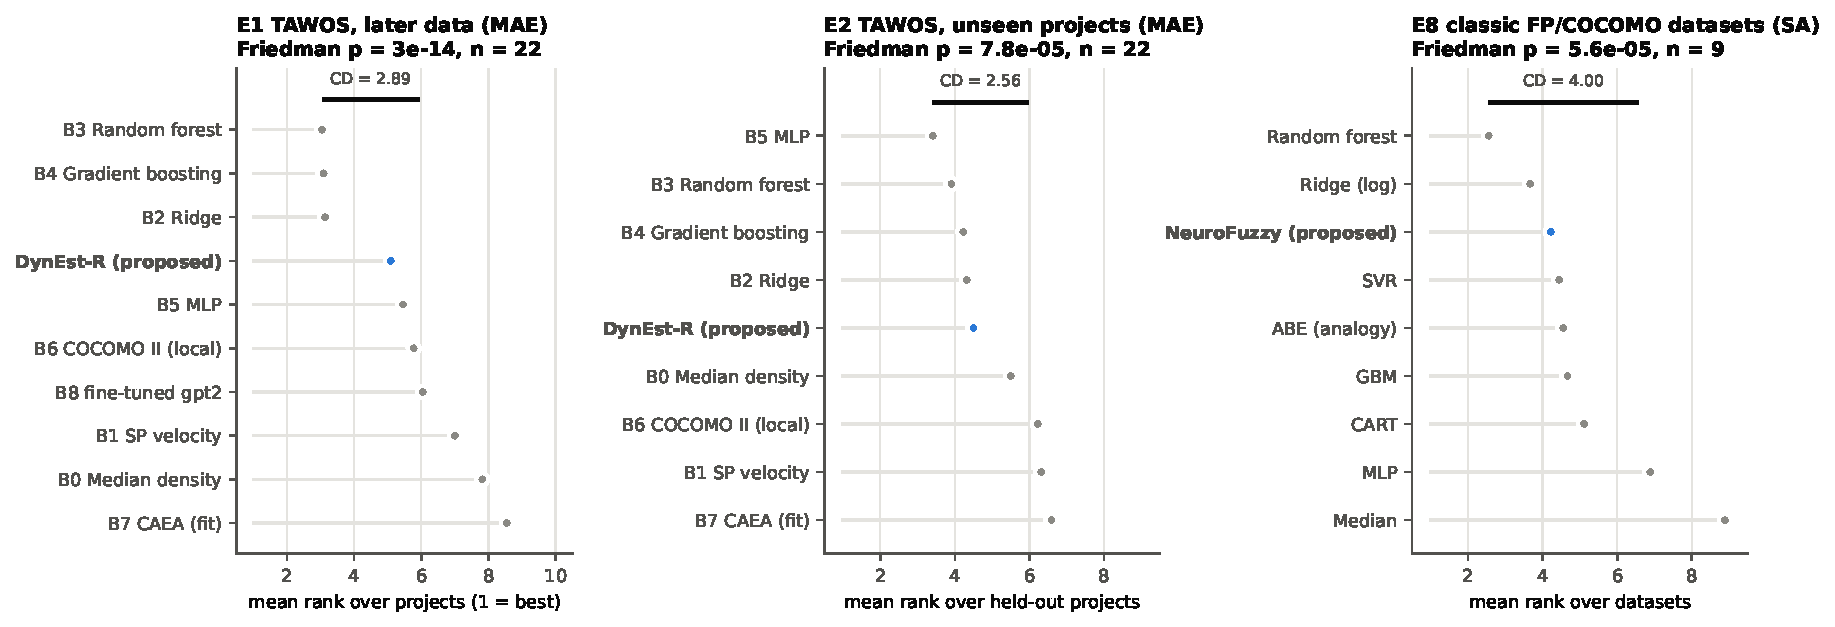
\includegraphics[width=\textwidth]{fig_ranks}
\caption{Mean ranks with Nemenyi critical differences (proposed models in blue).}
\label{fig:ranks}
\end{figure*}

\subsection{RQ2: unseen projects}
On leave-one-project-out (Table~\ref{tab:e2}) the full pipeline is within the group of tuned learners; differences to
ridge, random forest, gradient boosting and MLP are negligible and not significant, and it is ahead of story-point
velocity, COCOMO~II and CAEA on log error.  Its intervals keep their coverage on projects never seen (\ETwoCov).

\begin{table}[t]
\centering
\scriptsize
\caption{E2: accuracy on projects never seen in training (leave-one-project-out over 22 TAWOS projects).}
\label{tab:e2}
\begin{tabular}{lrrrrrrrrr}
\toprule
Model & MAE & MdAE & LMAE & SA & Cov. & IS & Rank & $r_{rb}$ MAE & $r_{rb}$ LMAE \\
\midrule
B5 MLP & 36.2 & 9.5 & 1.201 & 0.495 & -- & -- & 3.41 & +0.26 (1.000) & +0.37 (1.000) \\
B3 Random forest & 36.5 & 10.2 & 1.219 & 0.488 & -- & -- & 3.91 & +0.26 (1.000) & +0.45 (0.890) \\
B4 Gradient boosting & 36.4 & 10.3 & 1.216 & 0.490 & -- & -- & 4.23 & +0.24 (1.000) & +0.38 (1.000) \\
B2 Ridge & 36.8 & 10.8 & 1.228 & 0.487 & -- & -- & 4.32 & +0.15 (1.000) & +0.23 (1.000) \\
\textbf{DynEst-R (proposed)} & \textbf{36.6} & \textbf{10.1} & \textbf{1.233} & \textbf{0.486} & \textbf{0.945} & \textbf{622.78} & \textbf{4.50} & \textbf{--} & \textbf{--} \\
B0 Median density & 39.0 & 11.3 & 1.346 & 0.442 & -- & -- & 5.50 & -0.41 (1.000) & -0.51 (0.646) \\
B6 COCOMO II (local) & 37.4 & 12.3 & 1.299 & 0.471 & -- & -- & 6.23 & -0.60 (0.333) & -0.91 (0.001) \\
B1 SP velocity & 38.0 & 9.3 & 1.405 & 0.466 & -- & -- & 6.32 & -0.47 (1.000) & -0.77 (0.021) \\
B7 CAEA (fit) & 39.3 & 10.9 & 1.373 & 0.440 & -- & -- & 6.59 & -0.57 (0.447) & -0.72 (0.050) \\
\bottomrule
\end{tabular}
\par\smallskip\parbox{0.95\linewidth}{\footnotesize MAE/MdAE in hours; LMAE = mean $|\log(\hat y/y)|$; SA = standardised accuracy vs random guessing. Rank = mean rank of per-project MAE (Friedman $p$ = 7.8e-05, Nemenyi CD = 2.56, 22 projects). $r_{rb}$ = paired rank-biserial effect of the proposed model vs the row model on per-project error (negative = proposed better), Holm-adjusted $p$ in brackets (family: all baselines and ablations, as pre-registered). Cov. = coverage of the 95\% interval; IS = Winkler interval score relative to the mean actual (lower is better); every model's interval uses the same normalised Mondrian conformal recipe; a very large IS (COCOMO II) comes from a few extremely wide intervals where that model's residual-scale estimate is unstable, not from under-coverage.}
\end{table}


\subsection{RQ3: classic Function Point and COCOMO datasets}
Table~\ref{tab:e8} reports SA per dataset and Table~\ref{tab:e8-wtl} the per-dataset paired tests.  Random forest and
EBM have the best mean ranks; the neuro-fuzzy models are in the middle of a field in which all but the median and the
MLP lie within the critical difference.  On NASA93, which was not used to set COCOMO's constants, both neuro-fuzzy
models are clearly more accurate than COCOMO-81 with published constants and with local calibration; on COCOMO81
itself the published constants win, as expected, because they were fitted to those projects.  On Kitchenham the
recorded human first estimates are far more accurate than every model.

\begin{table}[t]
\centering
\scriptsize
\caption{E8: standardised accuracy (SA) on nine classic project-level datasets.}
\label{tab:e8}
\begin{tabular}{lrrrrrrrrrr}
\toprule
Model & Albrecht & Kemerer & Desharnai & China & Maxwell & Kitchenha & Miyazaki9 & COCOMO81 & NASA93 & Rank \\
\midrule
Random forest & 0.69 & \underline{0.52} & \underline{0.57} & 0.51 & 0.68 & 0.59 & 0.55 & 0.58 & \underline{0.73} & 2.56 \\
Ridge (log) & 0.70 & 0.47 & 0.56 & 0.52 & 0.61 & 0.55 & 0.52 & 0.77 & 0.68 & 3.67 \\
\textbf{NeuroFuzzy (proposed)} & \textbf{0.65} & \textbf{0.51} & \textbf{0.55} & \textbf{0.50} & \textbf{0.56} & \textbf{0.60} & \textbf{0.55} & \textbf{0.57} & \textbf{0.72} & \textbf{4.22} \\
SVR & 0.64 & 0.47 & 0.53 & 0.51 & 0.58 & \underline{0.60} & 0.54 & 0.74 & 0.68 & 4.44 \\
ABE (analogy) & \underline{0.73} & 0.51 & 0.56 & 0.46 & 0.53 & 0.54 & 0.53 & 0.64 & 0.73 & 4.56 \\
GBM & 0.69 & 0.39 & 0.53 & 0.51 & \underline{0.72} & 0.59 & 0.46 & 0.63 & 0.68 & 4.67 \\
CART & 0.69 & 0.51 & 0.55 & 0.48 & 0.62 & 0.60 & 0.44 & 0.53 & 0.65 & 5.11 \\
MLP & 0.56 & 0.35 & 0.50 & 0.47 & 0.39 & 0.52 & 0.53 & 0.76 & 0.63 & 6.89 \\
Median & 0.38 & 0.35 & 0.33 & 0.37 & 0.34 & 0.40 & 0.44 & 0.42 & 0.36 & 8.89 \\
COCOMO-81 local calib. & -- & -- & -- & -- & -- & -- & -- & 0.80 & 0.46 & -- \\
COCOMO-81 nominal & -- & -- & -- & -- & -- & -- & -- & \underline{0.84} & 0.50 & -- \\
COCOMO-81 refit & -- & -- & -- & -- & -- & -- & -- & 0.76 & 0.66 & -- \\
FP regression (log-log) & 0.71 & 0.49 & 0.50 & \underline{0.53} & 0.53 & 0.53 & -- & -- & -- & -- \\
KLOC power law (log-log) & -- & -- & -- & -- & -- & -- & \underline{0.56} & 0.61 & 0.58 & -- \\
\bottomrule
\end{tabular}
\par\smallskip\parbox{0.95\linewidth}{\footnotesize 3$\times$10-fold cross-validation, identical folds and tuning budget for every model; best per dataset underlined. Rank = mean SA rank over the datasets where every model applies (Friedman $p$ = 5.6e-05, Nemenyi CD = 4.00). COCOMO-81 variants need effort multipliers (COCOMO81, NASA93 only); Boehm calibrated the nominal constants on COCOMO81 itself.}
\end{table}

\begin{table}[t]
\centering
\small
\caption{E8: per-dataset win/tie/loss of the proposed model (Wilcoxon signed-rank on per-project absolute error, Holm-adjusted within dataset, $\alpha$ = 0.05).}
\label{tab:e8-wtl}
\begin{tabular}{lrrr}
\toprule
Proposed vs & Win & Tie & Loss \\
\midrule
KLOC power law (log-log) & 0 & 3 & 0 \\
CART & 1 & 8 & 0 \\
Median & 5 & 4 & 0 \\
ABE (analogy) & 0 & 8 & 1 \\
COCOMO-81 local calib. & 0 & 1 & 1 \\
COCOMO-81 nominal & 0 & 1 & 1 \\
COCOMO-81 refit & 0 & 1 & 1 \\
Expert first estimate (reference) & 0 & 0 & 1 \\
FP regression (log-log) & 0 & 5 & 1 \\
MLP & 2 & 6 & 1 \\
GBM & 0 & 7 & 2 \\
Ridge (log) & 0 & 7 & 2 \\
SVR & 0 & 7 & 2 \\
Random forest & 0 & 6 & 3 \\
\bottomrule
\end{tabular}
\end{table}


\subsection{RQ4: what each stage contributes}
On agile data every stage helps a little (Table~\ref{tab:ablation-tawos}, Figure~\ref{fig:ablation}); removing ANFIS
significantly worsens log error.  Learnt and expert rule bases are equally accurate, so the value of learning the
rules lies in not having to write them and in their agreement with data, not in accuracy.  On the small classic
datasets ANFIS alone is as good as or better than the full pipeline: with 15--100 projects the Mamdani partition
discards precision that the data cannot replace.

\begin{table}[t]
\centering
\small
\caption{E1 ablations: each stage of DynEst-R switched off (pooled test windows).}
\label{tab:ablation-tawos}
\begin{tabular}{lrrrr}
\toprule
Variant & MAE & $\Delta$MAE & LMAE & SA \\
\midrule
\textbf{DynEst-R (proposed)} & \textbf{52.41} & \textbf{--} & \textbf{1.226} & \textbf{0.368} \\
A5 no learned attributes & 52.56 & +0.3\% & 1.229 & 0.367 \\
A4 expert Mamdani (PBL rules) & 52.74 & +0.6\% & 1.219 & 0.365 \\
A1 no SOM & 52.94 & +1.0\% & 1.237 & 0.362 \\
A2 no ANFIS & 53.32 & +1.7\% & 1.303 & 0.358 \\
A3 no Mamdani & 53.61 & +2.3\% & 1.253 & 0.354 \\
\bottomrule
\end{tabular}
\end{table}


\begin{figure*}[t]
\centering
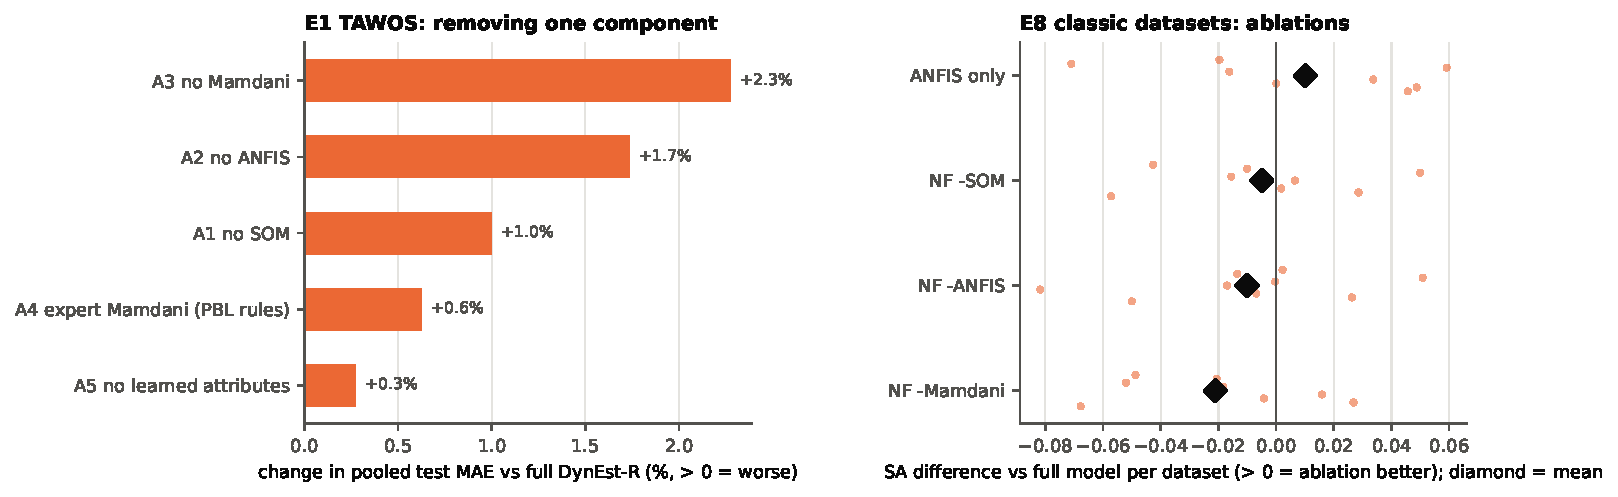
\includegraphics[width=\textwidth]{fig_ablation}
\caption{Ablations on agile data (left) and classic data (right).}
\label{fig:ablation}
\end{figure*}

\subsection{RQ5: uncertainty}
Given the same conformal recipe, every model's 95\% interval reaches nominal coverage on agile and classic data
(Figure~\ref{fig:intervals}); \dynest-T covers \ElevenCovT{} of test requirements.  Calibration is therefore a property
of the recipe, which we recommend for any estimator, rather than an advantage of the pipeline.  Intervals are wide
(median width about \ETwoWidth{} times the estimate on unseen projects), which reflects how noisy single-ticket
effort is and argues for aggregating estimates before committing.

\begin{figure*}[t]
\centering
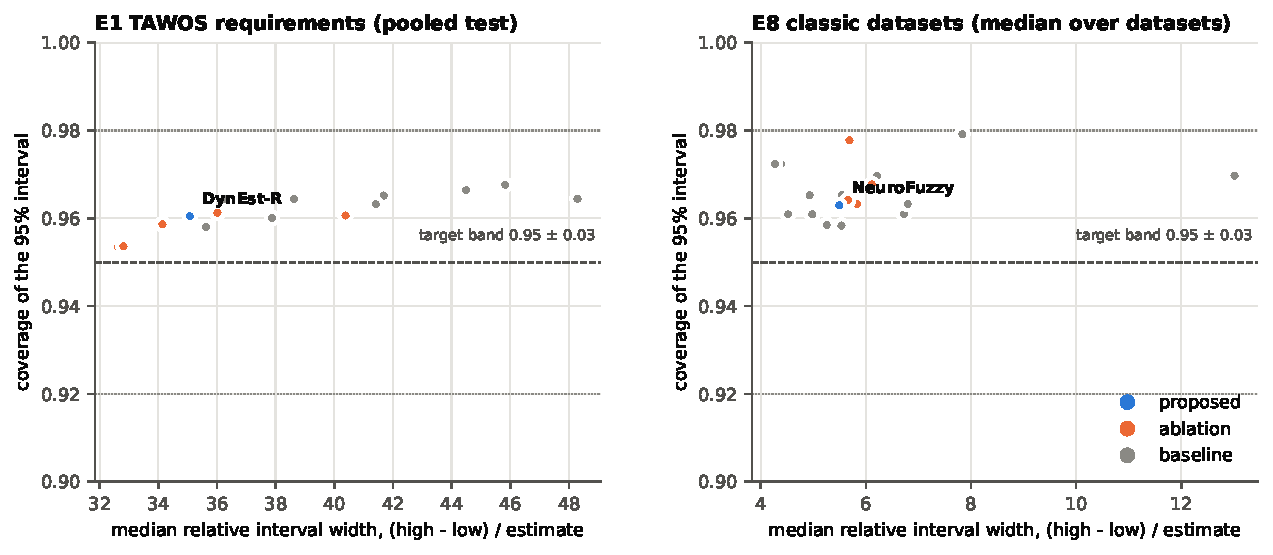
\includegraphics[width=\textwidth]{fig_intervals}
\caption{Coverage against width of the 95\% intervals; dashed line = nominal level.}
\label{fig:intervals}
\end{figure*}

\subsection{RQ6: are the rules readable and sensible?}
\dynest-T's rule base has \TRulesMin--\TRulesMax{} rules over three named inputs and covers every test requirement.
Before running E11 we declared the direction in which each readable input should move the estimate (slower similar
work, larger story-point counts per point, and lower familiarity should not decrease hours per point).  Of all pairs
of rules that differ by one linguistic term in one input, \TMonoMean\% move the consequent in the declared direction
or keep it (minimum \TMonoMin\% for any input and origin), although no such constraint was used in training.  For the
full pipeline, whose first input is the latent score, between \MonoMin\% and \MonoMax\% of neighbouring rules agree with
the analogous expectations, and \StableSame\% of shared antecedents keep their consequent across time origins
(Table~\ref{tab:e9}).  The SOM's topographic error is high (0.43--0.52) in this 30+-dimensional space, so the map is
best read as a source of priors rather than as a map of the requirement space.

\begin{table}[t]
\centering
\small
\caption{E9: size and quality of the learnt models per origin. $\le$3 rules = share of test requirements whose firing mass is $\ge$80\% in three rules; QE/TE = SOM quantisation and topographic error.}
\label{tab:e9}
\begin{tabular}{rrlrrrr}
\toprule
Origin & Rules & Terms & Coverage & $\le$3 rules & SOM QE & SOM TE \\
\midrule
0 & 36 & [4, 3, 3] & 1.00 & 0.37 & 3.33 & 0.52 \\
1 & 35 & [4, 3, 3] & 1.00 & 0.50 & 3.34 & 0.47 \\
2 & 27 & [3, 3, 3] & 1.00 & 0.52 & 3.39 & 0.43 \\
\bottomrule
\end{tabular}
\end{table}


\subsection{The pre-registered analysis}
\label{sec:prereg}
In the originally pre-registered experiment (E1), \dynest received 8 tuning trials and the baselines up to 40.  Its
pooled MAE was \EOneMAE{} hours and no baseline differed from it significantly after Holm correction over the
registered family (all baselines and ablations); it was significantly better than CAEA and median density.  Giving
\dynest five times more trials changed its validation error on the first origin by 0.2\% (45.72 to 45.62 hours), so
the budget gap did not hold the pipeline back; the stronger conclusion in E11 comes mainly from the smaller Holm
family (no ablations) and from the baselines that previously received 20 trials now receiving 40.  Table~S1 of the
supplementary material reports E1 in full.

%==================================================================================================
\section{Discussion}
\label{sec:discussion}

\paragraph{What transparency costs.}  On 22 agile projects, a rule base that a team lead can read in full (three
named inputs, a few dozen rules) is about one per cent less accurate than the best tuned black-box learner, the same
price as the leading glass-box alternative (EBM), and the per-project differences are consistent enough to be
statistically detectable.  Whether one per cent matters depends on use: against an irreducible error of roughly 0.8
on the relative scale, it is small, and a model whose every estimate can be traced to two or three fired rules may be
worth it where estimates must be justified to stakeholders.  The fuzzy rule base and EBM offer different kinds of
transparency: EBM shows one shape function per feature and pairwise interactions; the Mamdani base states conditions
in words and allows a reviewer to check a rule against experience.

\paragraph{Where the effort is in the pipeline.}  The SOM prior is the strongest readable input; it encodes
``requirements like this one took this many hours per point in this project'', which is how experienced estimators
reason.  The multi-stage structure helps on large data and not on small data, where ANFIS alone is enough.

\paragraph{Uncertainty is cheap and should be standard.}  The same conformal recipe calibrated every model,
including the weakest; reporting intervals therefore needs no special model.  The width of the intervals is itself a
finding: at the level of a single ticket, effort is too noisy for point estimates to be relied on.

\paragraph{Text models are not the answer on this target.}  Fine-tuned GPT-2 and DeBERTa-v3, given the same
decision-time text and metadata, did not beat ridge regression on measured features.  This agrees with replications
of story-point models~\citep{tawosi2023deepse,tawosi2022gpt2sprep} and extends them to effort in hours.

\paragraph{For researchers.}  Three practices changed our conclusions and should be routine: reconstructing features
as of decision time; giving every model the same tuning budget (our first analysis gave the baselines five times our
budget); and giving every model the same interval method before comparing uncertainty.

%==================================================================================================
\section{Threats to validity}
\label{sec:threats}
\emph{Construct.}  Effort on agile data is a measured proxy; its validity is moderate ($\rho\approx\ProxyRho$) and we
report it rather than assume it.  Status semantics differ across projects; the active-status rule is a measurement
definition.  Interpretability is measured by rule-base properties and agreement with declared expectations; whether
the explanations help practitioners judge estimates has not yet been tested with users.
\emph{Internal.}  The equal-budget experiment, the transparent variant and three baselines were added after the
pre-registered results were seen;
we report both analyses and recorded the amendment before running it.  On classic data the transparent variant may
choose one-hot indicator variables as fuzzy inputs, which adds little; the agile variant excludes them.  CAEA's
published constants were not transcribed; only a fitted CAEA is reported.  Large language models were not evaluated.
\emph{External.}  Open-source projects only; the classic datasets are old and small.
\emph{Conclusion.}  Many comparisons; we correct with Holm and report paired effect sizes and confidence intervals.

\section{Conclusion}
\label{sec:conclusion}
A neuro-fuzzy estimator whose rules, partitions, clusters and back-transform are all learnt from real data can explain
every estimate with a few dozen readable rules over named inputs, give calibrated intervals, and stay within about one
per cent of the best tuned black-box learner on real agile histories, at the same cost as the leading glass-box
alternative.  It does not beat the best black boxes, and we found no evidence that larger text models would change
that on this target.  Future work: monotonicity-constrained rule learning, a practitioner study of the rules, and a
public decision-time benchmark for text-based and LLM estimators.

\section*{Data and code availability}
Code, configuration, pre-registered endpoints and the amendment, and all result tables are available at
\todo{repository / Zenodo DOI}.  TAWOS must be obtained from its authors; the classic datasets are downloaded by a
script from public PROMISE copies.

\bibliographystyle{elsarticle-harv}
\bibliography{refs}

\end{document}
